\documentclass{standalone}
\usepackage{tikz}
\tikzset{point/.style={circle,draw=black,inner sep=0pt,minimum size=3pt}}
\usepackage{tikz}
\usetikzlibrary{calc}
\usetikzlibrary{arrows,graphs,matrix,positioning, arrows.meta, automata}

\begin{document}

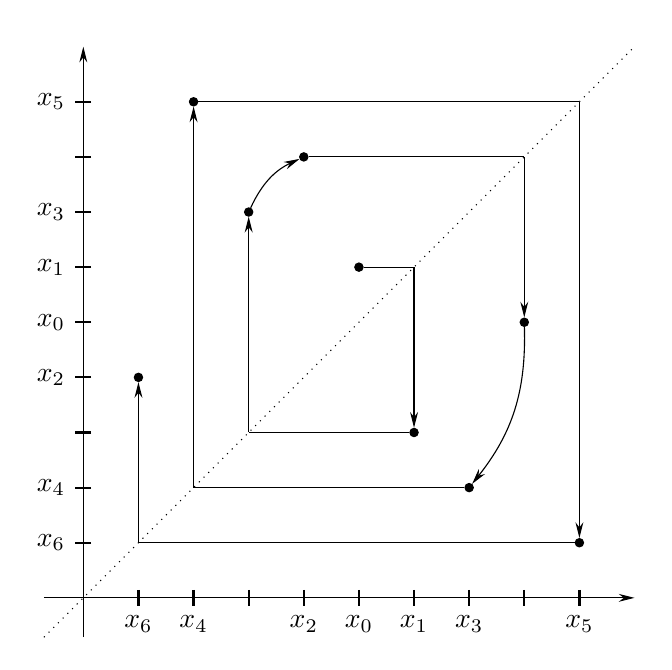
\begin{tikzpicture}[>={Stealth[length=2mm, width=1mm]}]

\draw[->] (-0.5, 0) -- (7, 0) node[below] {};
\draw[->] (0, -0.5) -- (0, 7) node[above] {};
\node[point,fill=black] (a) at (0.7,2.8) {};
\node[point,fill=black] (b) at (1.4,6.3) {};
\node[point,fill=black] (c) at (2.1,4.9) {};
\node[point,fill=black] (d) at (2.8,5.6) {};
\node[point,fill=black] (e) at (3.5,4.2) {};
\node[point,fill=black] (f) at (4.2,2.1) {};
\node[point,fill=black] (g) at (4.9,1.4) {};
\node[point,fill=black] (h) at (5.6,3.5) {};
\node[point,fill=black] (i) at (6.3,0.7) {};

\draw (e) -- (f|-e);
\draw[->] (f|-e) -- (f);
\draw (f) -- (c|-f);
\draw[->] (c|-f) -- (c);
\draw[->] (c) to[bend left=20] (d);
\draw (d) -- (h|-d);
\draw[->] (h|-d) -- (h);
\draw[->] (h) to[bend left=20] (g);
\draw (g) -- (b|-g);
\draw[->] (b|-g) -- (b);
\draw (b) -- (i|-b);
\draw[->] (i|-b) -- (i);
\draw (i) -- (a|-i);
\draw[->] (a|-i) -- (a);

\draw[dotted] (-0.5, -0.5) -- (7, 7);

\draw[thick] (0.1,0 |-a) -- (-0.1,0 |-a) node[left] {$x_2$};
\draw[thick] (0.1,0 |-b) -- (-0.1,0 |-b) node[left] {$x_5$};
\draw[thick] (0.1,0 |-c) -- (-0.1,0 |-c) node[left] {$x_3$};
\draw[thick] (0.1,0 |-d) -- (-0.1,0 |-d);
\draw[thick] (0.1,0 |-e) -- (-0.1,0 |-e) node[left] {$x_1$};
\draw[thick] (0.1,0 |-f) -- (-0.1,0 |-f);
\draw[thick] (0.1,0 |-g) -- (-0.1,0 |-g) node[left] {$x_4$};
\draw[thick] (0.1,0 |-h) -- (-0.1,0 |-h) node[left] {$x_0$};
\draw[thick] (0.1,0 |-i) -- (-0.1,0 |-i) node[left] {$x_6$};

\draw[thick] (a |- 0,0.1) -- (a |- 0,-0.1) node[below] {$x_6$};
\draw[thick] (b |- 0,0.1) -- (b |- 0,-0.1) node[below] {$x_4$};
\draw[thick] (c |- 0,0.1) -- (c |- 0,-0.1);
\draw[thick] (d |- 0,0.1) -- (d |- 0,-0.1) node[below] {$x_2$};
\draw[thick] (e |- 0,0.1) -- (e |- 0,-0.1) node[below] {$x_0$};
\draw[thick] (f |- 0,0.1) -- (f |- 0,-0.1) node[below] {$x_1$};
\draw[thick] (g |- 0,0.1) -- (g |- 0,-0.1) node[below] {$x_3$};
\draw[thick] (h |- 0,0.1) -- (h |- 0,-0.1);
\draw[thick] (i |- 0,0.1) -- (i |- 0,-0.1) node[below] {$x_5$};

%    \draw[dotted,thick] (b) -- (b|-origin) node[below] {$b$};
%    \draw[dotted,thick] (a) -- (origin |-a) node[left] {$f(a)$};
%     \draw[dotted,thick] (b) -- (origin |-b) node[left] {$f(b)$};
\end{tikzpicture}
\end{document}